\documentclass[a4paper]{article}
\usepackage[UTF8]{ctex}
\usepackage[colorlinks, linkcolor=blue]{hyperref}
\usepackage[a4paper, top=2cm, bottom=1.5cm, left=2.5cm, right=2.5cm]{geometry}
\usepackage{enumerate, tcolorbox, amsmath, booktabs, fontspec, tikz, harmony}

\usepackage{fancyhdr}
\pagestyle{fancy}
\fancyhf{}
\fancyfoot[L]{
    
\includegraphics[height=2\baselineskip]{assets/Logo(1).png}
    \begin{tabular}[b]{l}
        欢迎加入 \href{https://github.com/manim-kindergarten}{\texttt{Manim Kindergarten}}\\
        一起来玩 \href{https://github.com/manim-kindergarten/manim_sandbox}{\texttt{Manim Sandbox}}
    \end{tabular}
}
\fancyfoot[R]{\normalsize\thepage}
\renewcommand{\footrulewidth}{0.5pt}
\renewcommand{\headrulewidth}{0.5pt}

\usepackage{listings}
\lstset{
	basicstyle=\fontspec{Consolas}
}

\begin{document}

\vspace*{50mm}
\begin{center}
    \huge manim 常见问题 v2.2 \\
    \LARGE 鹤翔万里\& catfish \\
    \today
\end{center}

\newpage

\begin{center}
    \tableofcontents
\end{center} 

\newpage

\begin{center}
    \section{安装问题}
\end{center}

安装时最好不要看\texttt{README.md}自己研究,
推荐一视数学卷毛杨的两个教程:
\begin{itemize}
    \item \url{https://www.bilibili.com/video/av38126904}
    \item \url{https://www.bilibili.com/read/cv4139851}
\end{itemize}

\subsection{\texttt{Python}问题}
\subsubsection*{Q1: 使用\texttt{anaconda},命令行输入\texttt{python}无反应或报错}

考虑\texttt{path}环境变量是否填全\footnote{安装\texttt{anaconda}时是否勾选添加到\texttt{path}变量},\texttt{path}变量里应该有:

\begin{verbatim}
    <your_path>\Anaconda3;
    <your_path>\Anaconda3\Scripts;
    <your_path>\Anaconda3\Library\bin;
\end{verbatim}

\subsubsection*{Q2: \texttt{pip install ...}时满屏红字报错,或者安装过慢}

更换国内镜像源,使用 
\begin{verbatim}
    pip install -r requirements.txt -i https://pypi.tuna.tsinghua.edu.cn/simple
\end{verbatim}

代替\footnote{临时换源}
\begin{verbatim}
    pip install -r requirements.txt
\end{verbatim}

\subsubsection*{Q3: \texttt{pip}安装\texttt{pycairo}总是失败}

下载\texttt{pycairo}对应版本的\texttt{whl}包
\footnote{群文件中有某个版本的\texttt{pycairo},注意\texttt{Python}版本和系统版本是否均合适}
\begin{verbatim}
    pycairo......whl
\end{verbatim}

并手动安装
\begin{verbatim}
    pip install pycairo......whl
\end{verbatim}

\subsubsection*{Q4: \texttt{pip}安装过包,但运行时提示没有模块}
考虑电脑上是否有多个\texttt{Python},确定\texttt{pip}把包装到了需要使用的\texttt{Python}上面。

\newpage

\begin{center}
    \section{运行时问题}
\end{center}

\subsection{\texttt{import}问题}
\subsubsection*{Q1: 没有模块\texttt{big\_ol\_pile\_of\_manim\_imports}}

将文件中的
\begin{verbatim}
    from big_ol_pile_of_manim_imports import *
\end{verbatim}

改成
\begin{verbatim}
    from manimlib.imports import *
\end{verbatim}

\subsection{\LaTeX 问题}
\subsubsection*{Q1: 报错\texttt{Latex error converting to dvi}}
先不要管错误在哪,先把\texttt{manimlib/constants.py}中的\texttt{TEX\_USE\_CTEX}改成\texttt{True}再运行

\subsubsection*{Q2: 报错 \texttt{xelatex error converting to xdv}}\label{sub:Q2}
若为\texttt{Windows}系统,先把\texttt{manimlib/constants.py}的第29行:
\begin{verbatim}
    MEDIA_DIR = "./media"
\end{verbatim}

改成
\begin{verbatim}
    MEDIA_DIR = os.path.join(os.getcwd(), "media")
\end{verbatim}

再进行尝试

\begin{enumerate}[I.]
    \item \textbf{若安装的\texttt{\TeX}发行版为\texttt{MiK\TeX}}
    \begin{enumerate}[1.]
        \item \texttt{MiK\TeX}的有关路径是否添加到环境变量中
        \item 是否有包没有装全
    \end{enumerate}

    \begin{tcolorbox}
        对于\texttt{2.},可以正常运行一遍\texttt{WriteStuff}场景,看是否有框弹出提示\texttt{install}什么东西,
        如果有,则\texttt{install},并重复运行安装运行安装...直到不报错为止。 \\
        或者使用\TeX 编辑器\texttt{\TeX Studio}
        并使用\texttt{xelatex}手动编译\texttt{media/Tex}文件夹中的{} \texttt{.tex}文件,查看是否有包没有安装。
    \end{tcolorbox}
        
    \begin{tcolorbox}
        对于没有\texttt{1.}和\texttt{2.}问题却依旧报错的,可以选择重新安装新版\texttt{MiK\TeX}或者安装\texttt{\TeX Live-full}版。
    \end{tcolorbox}

    \item \textbf{若安装的\texttt{\TeX}发行版为\texttt{\TeX Live}}
    \begin{enumerate}[1.]
        \item \texttt{\TeX Live}有关路径是否添加到环境变量中
        \item 安装的是否为\texttt{full}版本
    \end{enumerate}

    \item \textbf{若安装的\texttt{\TeX}发行版不为以上两款}
    
    建议换成\texttt{\TeX Live-full}版或者\texttt{MiK\TeX},并且在重新安装前请删除旧版
\end{enumerate}

\subsubsection*{Q3: 报错在文件夹内找不到\texttt{svg}文件}

清空\texttt{media/Tex}文件夹内全部内容,再次运行带文字的场景,查看\texttt{Tex}文件夹中的内容:

\begin{enumerate}[I.]
    \item 若仅有\texttt{tex}文件和\texttt{log}文件,按照\texttt{\ref{sub:Q2}}中方法处理
    \item 若含有\texttt{xdv}文件但没有\texttt{svg}文件
    \begin{enumerate}[1.]
        \item \texttt{divsvgm}是否添加到环境变量,可以使用\texttt{dvisvgm --version}观察是否由报错来检查
        \item \texttt{dvisvgm}版本是否过低,若\texttt{dvisvgm --verison}的输出版本号为1开头,\\
        请更换新版\texttt{dvisvgm}\footnote{上网下载、或者使用群文件中的版本},并注意将含有\texttt{dvisvgm}的文件夹添加到环境变量中
    \end{enumerate}
\end{enumerate}

\subsection{中文显示问题}
\subsubsection*{Q1: 含有中文的\texttt{TextMobject}编译报错,\texttt{Latex error converting to dvi}}

将\texttt{manimlib/constants.py}中的\texttt{TEX\_USE\_CTEX}改成\texttt{True}再尝试

\subsubsection*{Q2: 英文可以正常显示,中文不报错,但不显示}

考虑使用的是否为\texttt{TextMobject}而不是\texttt{TexMobject}

\subsection{文字问题}
\subsubsection*{Q1: \texttt{TextMobject}和\texttt{TexMobject}有什么区别}

\texttt{TextMobject}和\texttt{TexMobject}使用的都是\LaTeX 语法

其中\texttt{TextMobject}文字模式相当于直接在\LaTeX 环境下书写

\texttt{TexMobject}公式模式使用的是\LaTeX 的 \texttt{\textbackslash begin\{align*\}}
环境或者可以看成加了$\texttt{\$}\texttt{\$}$的环境

使用\texttt{TextMobject}与\texttt{TexMobject}书写公式时:

\fbox{$\texttt{TextMobject("} \text{文字} \texttt{\$} \text{公式} \texttt{\$")} \Longleftrightarrow \texttt{TexMobject("\textbackslash \textbackslash text\{} \text{文字} \texttt{\}} \text{公式} \texttt{")}$}

\subsubsection*{Q2: \texttt{TextMobject}中怎么改字体样式}

\texttt{TextMobject}中只能使用\LaTeX 的字体样式

字体常用样式命令见表:
\begin{table}[htbp]
    \centering
    \begin{tabular}{llll}
        \toprule
        字体样式 & \LaTeX 命令  & 字体样式 & \LaTeX 命令 \\
        \midrule
        \textrm{roman}  & \texttt{\textbackslash textrm\{\dots\}} & \textbf{bold face} & \texttt{\textbackslash textbf\{\dots\}} \\
        \textsf{sans serif} & \texttt{\textbackslash textsf\{\dots\}} & \textmd{medium weight} & \texttt{\textbackslash textmd\{\dots\}} \\
        \texttt{typewriter} & \texttt{\textbackslash texttt\{\dots\}} & \textit{italic} & \texttt{\textbackslash textit\{\dots\}} \\
        \textsc{Small Caps} & \texttt{\textbackslash textsc\{\dots\}} & \textsl{slanted} & \texttt{\textbackslash textsl\{\dots\}} \\
        \textup{upright} & \texttt{\textbackslash textup\{\dots\}} \\
        \bottomrule
    \end{tabular}
\end{table}

严格地讲中文字体并没有衬线、无衬线、等宽、斜体等概念

\subsubsection*{Q3: 想自定义字体怎么办}

使用新版\texttt{manim}特有的\texttt{Text()}类,
方法如下$\texttt{Text("}\text{文字}\texttt{", font="}\text{字体}\texttt{")}$,
其中字体要填写在计算机内存储的格式\footnote{例如:Microsoft YaHei,Source Han Sans CN},但是不能使用\LaTeX 语法书写公式

\subsubsection*{Q4: 想用自定义字体写公式怎么办}

可以使用群文件里\texttt{cigar666}编写的\texttt{MyText()}类$_{\text{\texttt{Cigar}牛逼}}$

\subsubsection*{Q5: \texttt{TexMobject}中换行是什么}
四个右划线\texttt{\textbackslash \textbackslash \textbackslash \textbackslash},
\texttt{Python}转义右划线,所以涉及到\texttt{\textbackslash}的均要写成两个\texttt{\textbackslash \textbackslash},
而换行在\LaTeX 中是两个右划线,所以要写成四个\footnote{或者在字符串前加r,正常书写}

\subsubsection*{Q6: 公式怎么对齐}
\begin{enumerate}[I.]
    \item 直接在\texttt{TexMobject}中使用\texttt{\&}对齐
    \item 两个\texttt{mobject}对齐,使用\texttt{obj2.next\_to(obj1, DOWN, aligned\_edge=LEFT)}使\texttt{obj2}在\texttt{obj1}下方,并左对齐
    \item \texttt{VGroup}内对齐,使用\texttt{group.arrange(DOWN, aligned\_edge=LEFT)}使\texttt{VGroup}中的子元素依次向下排开,并左对齐
\end{enumerate}

写公式的示例:

\url{https://github.com/Elteoremadebeethoven/AnimationsWithManim/blob/master/English/3_text_like_arrays/scenes.md}

\subsubsection*{Q7: \texttt{TexMobject}上色问题的处理办法}
\begin{enumerate}[I.]
    \item 将上色的字符分开,使用\texttt{text[i].set\_color(color)} 来上色
    \item 将上色的字符分开,使用\texttt{text.set\_color\_by\_tex\_to\_color\_map(t2c)}传入\texttt{t2c}字典来对相同的字符串上色
    \item 只传入一个字符串,但同时传入\texttt{tex\_to\_color\_map=t2c}来自动拆分上色(容易出问题)
    \item 只传入一个字符串,使用\texttt{text[0][i]}来对细小的路径上色(一般是一个字符一个下标)
\end{enumerate}

\subsubsection*{Q8: \texttt{TexMobject}的下标怎么分析}

创建函数

\begin{lstlisting}
def debugTeX(self, texm):
    for i, j in zip(range(100), texm):
        tex_id = TextMobject(str(i)).scale(0.3).set_color(PURPLE)
        tex_id.move_to(j)
        self.add(tex_id)
\end{lstlisting}

在使用时先\texttt{self.add(tex)}然后再\texttt{debugTeX(self, tex)},
导出最后一帧\footnote{-s 选项},观察每段字符上的标号,即为下标

\subsubsection*{Q9: \texttt{TexMobject}使用 \texttt{\textbackslash frac} 拆分时出错}
这个是\texttt{Grant}写\texttt{tex\_file\_writing.py} 的一个\texttt{bug},
建议使用\texttt{\{}分子 \texttt{\textbackslash over}分母\texttt{\}}
来代替 \texttt{\textbackslash frac\{}分子\texttt{\}\{}分母\texttt{\}}

\subsubsection*{Q10: 括号匹配不全}
显示不全的例子:$\left\{\begin{matrix}
    a+b \\
    b+a \\
\end{matrix}\right.$
\begin{verbatim}
    TexMobject(r"\left\{\begin{matrix} a+b \\ b+a \\ \end{matrix}\right.")
\end{verbatim}

\texttt{matrix}这样的写法在\texttt{manim}中会报错,无法生成\texttt{dvi},
原因是\texttt{manim}会自动寻找相对应的括号来匹配,这里缺少了右边的大括号

所以推荐使用\texttt{cases}环境,效果是一样的:$\begin{cases}
    a+b \\
    b+a \\
\end{cases}$
\begin{verbatim}
    TexMobject(r"\begin{cases} a+b \\ b+a \\ \end{cases}")
\end{verbatim}

\subsection{素材引用问题}
\subsubsection*{Q1: 使用\texttt{SVGMobject}找不到\texttt{svg}文件}
\begin{enumerate}[I.]
    \item 直接使用绝对路径引用\texttt{svg}文件
    \item 将\texttt{svg}文件放到\texttt{assets/svg\_images/}文件夹中
\end{enumerate}

\subsubsection*{Q2: 如何使用\texttt{jpg}或者\texttt{png}文件}
\begin{enumerate}[I.]
    \item 直接使用绝对路径引用,并使用\texttt{ImageMobject}
    \item 将\texttt{jpg/png}文件放到\texttt{assets/raster\_images/}文件夹中
\end{enumerate}

\begin{center}
    \section{其它问题}
\end{center}

\subsection*{Q1: 有什么manim教程}
\addcontentsline{toc}{subsection}{Q1: 有什么\texttt{manim}教程}
\begin{enumerate}[1.]
    \item 群主\texttt{cigar666}的B站专栏
    \begin{itemize}
        \item \url{https://www.bilibili.com/read/readlist/rl82339}
    \end{itemize}
    \item \texttt{pdcxs}大大转载的\texttt{manim}教程
    \begin{itemize}
        \item \url{https://www.bilibili.com/video/av64023740}
        \item 源码 \url{https://github.com/Elteoremadebeethoven/AnimationsWithManim}
    \end{itemize}
    \item \texttt{GitHub}上\texttt{cai-hust}的中文教程
    \begin{itemize}
        \item \url{https://github.com/cai-hust/manim-tutorial-CN}
    \end{itemize}
    \item 看\texttt{manim}源码
\end{enumerate}

\subsubsection*{Q2: 没有\texttt{manim}源码}
\addcontentsline{toc}{subsection}{Q2: 没有\texttt{manim}源码}
最好不要使用\texttt{pip install manimlib}来装\texttt{manim},请在\texttt{GitHub}上\texttt{clone}下来\texttt{manim}的全部内容

\newpage

\subsubsection*{Q3: 群友用的\texttt{manim}都是什么版本}
\addcontentsline{toc}{subsection}{Q3: 群友用的\texttt{manim}都是什么版本}
\texttt{manim}不看版本,一般使用的都是最新库,\texttt{release}里面带版本号的都可以看作旧版

\subsubsection*{Q4: 如何使用傅里叶级数作图}
\addcontentsline{toc}{subsection}{Q4: 如何使用傅里叶级数作图}
套用 Grant 写好的文件
\begin{verbatim}
    active_projects/diffyq/part2/fourier_series.py
    active_projects/diffyq/part4/fourier_series_scenes.py
    active_projects/diffyq/part4/long_fourier_series.py
\end{verbatim}

只需要更换\texttt{svg}素材即可\footnote{自己制作,或者使用群里的\texttt{svg}素材}

\subsubsection*{Q5: \texttt{svg}用什么软件制作}
\addcontentsline{toc}{subsection}{Q5: \texttt{svg}用什么软件制作}
\texttt{Adobe Illustrator}(简称 AI)或者\texttt{inkscape}(简称 ink)

尽量不要使用网页版编辑器

\subsubsection*{Q6: 动画怎么显示旋转一个物体}
\addcontentsline{toc}{subsection}{Q6: 动画怎么显示旋转一个物体}
使用\texttt{Ratate}和\texttt{Rotating},区别在群文件中有视频

\subsubsection*{Q7: 怎么控制物体移动或者\texttt{Transform}的加速度}
\addcontentsline{toc}{subsection}{Q7: 怎么控制物体移动或者\texttt{Transform}的加速度}
使用\texttt{rate\_func},一些\texttt{manim}中已经定义的在群文件中有视频

\begin{figure}[htbp]
    \begin{minipage}{0.18\linewidth}
        \centerline{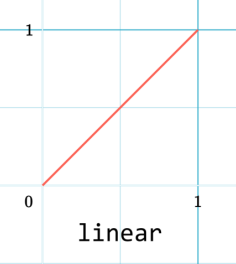
\includegraphics[width=1in]{assets/linear.png}}    
    \end{minipage}
    \begin{minipage}{0.18\linewidth}
        \centerline{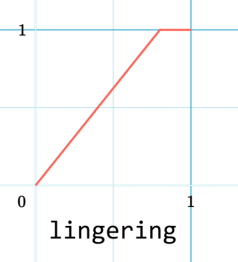
\includegraphics[width=1in]{assets/lingering.png}}    
    \end{minipage}
    \begin{minipage}{0.18\linewidth}
        \centerline{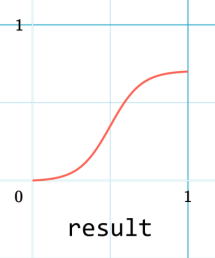
\includegraphics[width=1in]{assets/result.png}}    
    \end{minipage}
    \begin{minipage}{0.18\linewidth}
        \centerline{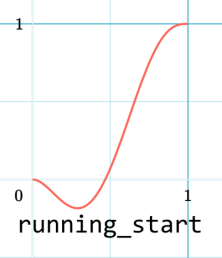
\includegraphics[width=1in]{assets/running_start.png}}    
    \end{minipage}
    \begin{minipage}{0.18\linewidth}
        \centerline{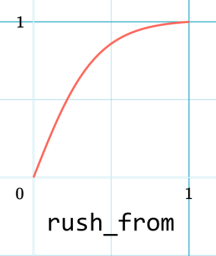
\includegraphics[width=1in]{assets/rush_from.png}}    
    \end{minipage}
\end{figure}

\begin{figure}[htbp]
    \begin{minipage}{0.18\linewidth}
        \centerline{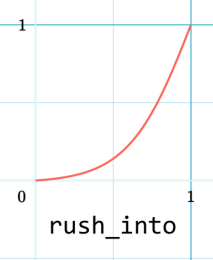
\includegraphics[width=1in]{assets/rush_into.png}}    
    \end{minipage}
    \begin{minipage}{0.18\linewidth}
        \centerline{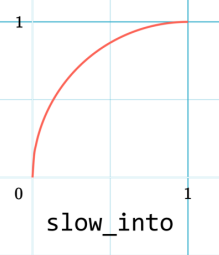
\includegraphics[width=1in]{assets/slow_into.png}}    
    \end{minipage}
    \begin{minipage}{0.18\linewidth}
        \centerline{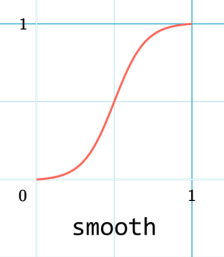
\includegraphics[width=1in]{assets/smooth.png}}    
    \end{minipage}
    \begin{minipage}{0.18\linewidth}
        \centerline{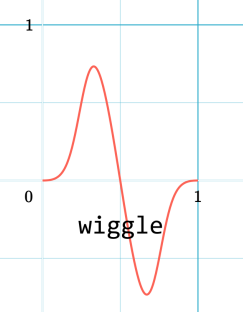
\includegraphics[width=1in]{assets/wiggle.png}}    
    \end{minipage}
    \begin{minipage}{0.18\linewidth}
        \centerline{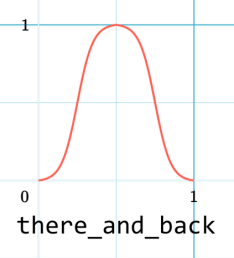
\includegraphics[width=1in]{assets/there_and_back.png}}    
    \end{minipage}
\end{figure}

\begin{figure}[htbp]
    \begin{minipage}{0.18\linewidth}
        \centerline{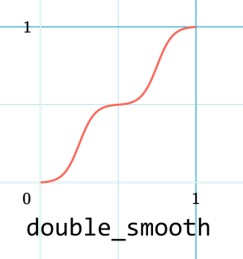
\includegraphics[width=1in]{assets/double_smooth.png}}    
    \end{minipage}
    \begin{minipage}{0.2\linewidth}
        \centerline{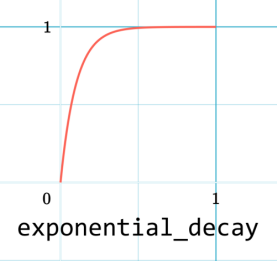
\includegraphics[width=1.2in]{assets/exponential_decay.png}}    
    \end{minipage}
    \begin{minipage}{0.3\linewidth}
        \centerline{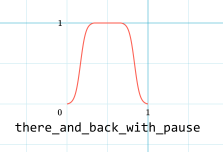
\includegraphics[width=1.8in]{assets/there_and_back_with_pause.png}}    
    \end{minipage}
\end{figure}

\newpage

\subsubsection*{Q8: 数学符号/公式 用\LaTeX 怎么打}
\addcontentsline{toc}{subsection}{Q8: 数学符号\texttt{/}公式 用\LaTeX 怎么打}
请见 \url{https://www.luogu.com.cn/blog/IowaBattleship/latex-gong-shi-tai-quan}

\subsubsection*{Q9: 一些特殊\LaTeX 的外部包}
\addcontentsline{toc}{subsection}{Q9: 一些特殊\LaTeX 的外部包}

\Ganz \Halb \Vier \Acht \Sech \Zwdr

\textbf{如何使用\texttt{manim}画出上面的音符,或怎么使用这些包?}

在\texttt{manimlib}目录下的\texttt{ctex\_template.tex}或者\texttt{tex\_template.tex}文件中
添加外部包的名称\footnote{修改\texttt{TEX\_USE\_CTEX}为\texttt{True}的,可以只在\texttt{ctex\_template.tex}中添加}

就拿上面的音符为例,因为是在\texttt{harmony}包中的,所以在\texttt{tex}文件中添加\texttt{\textbackslash usepackage\{harmony\}}\footnote{不需要使用的时候记得改回来哦\label{change}}

然后新建一个\texttt{py}文件,写入代码
\begin{lstlisting}
    from manimlib.imports import *
    class TestHarmony(Scene):
        def construct(self):
            # harmony具体用法请百度
            harmony = TextMobject(r"\Ganz \Halb \Vier \Acht \Sech \Zwdr")
            self.play(ShowCreation(harmony))
            self.wait()
\end{lstlisting}

运行py文件即可

\subsubsection*{Q10: 使用\LaTeX 外部包,编译错误或者无显示}
\addcontentsline{toc}{subsection}{Q10: 使用\LaTeX 外部包,编译错误或者无显示}
首先,并不是所有外部包都能在\texttt{manim}中顺利使用,大多都不支持\texttt{xelatex}编译,
所以建议需要使用外部包时只用\texttt{latex}编译\footnote{即把\texttt{TEX\_USE\_CTEX}改为\texttt{False}}

至于有些群友常用\texttt{tiKz}这个外部包,也是使用\texttt{latex}才能顺利运行,
在\texttt{xelatex}用{} \texttt{\textbackslash draw}会无法显示,
需要修改\texttt{tex\_template.tex}文件\textsuperscript{\ref{change}},修改成如下:

\begin{lstlisting}
    \documentclass[preview, dvisvgm]{standalone}
    \usepackage{tikz}
\end{lstlisting}

新建\texttt{py}文件,写入代码来画一条线:\begin{tikzpicture}
    \draw (-1, 0) -- (1, 0);
\end{tikzpicture}

\begin{lstlisting}
    class TestTikz(Scene):
        def construct(self):
            tikz = TextMobject(
                # tikz具体用法请百度
                r"\tikz{\draw (-1, 0) -- (1, 0);}",
                color=WHITE,
                stroke_width=1,
                stroke_opacity=1,
            )
            self.play(ShowCreation(tikz))
            self.wait()
\end{lstlisting}

运行py文件即可

\subsubsection*{Q11: 一些比较复杂,操纵东西比较多的动画怎么做}
\addcontentsline{toc}{subsection}{Q11: 一些比较复杂,操纵东西比较多的动画怎么做}
使用外部剪辑软件,例如\texttt{Adobe Premiere Pro}或者达芬奇

\subsubsection*{Q12: 一个\texttt{self.play}里写两个\texttt{ApplyMethod}只对一个起作用怎么办}
\addcontentsline{toc}{subsection}{Q12: 一个\texttt{self.play}里写两个\texttt{ApplyMethod}只对一个起作用怎么办}
去掉\texttt{ApplyMethod}

\subsubsection*{Q13: 如何解决二维画面中的图层问题}
\addcontentsline{toc}{subsection}{Q13: 如何解决二维画面中的图层问题}
使用z轴坐标对图层进行区分是无效的

可以使用\texttt{pdcxs}添加的\texttt{plot\_depth},具体更改见下图
\begin{figure}[h]
	\begin{center}
		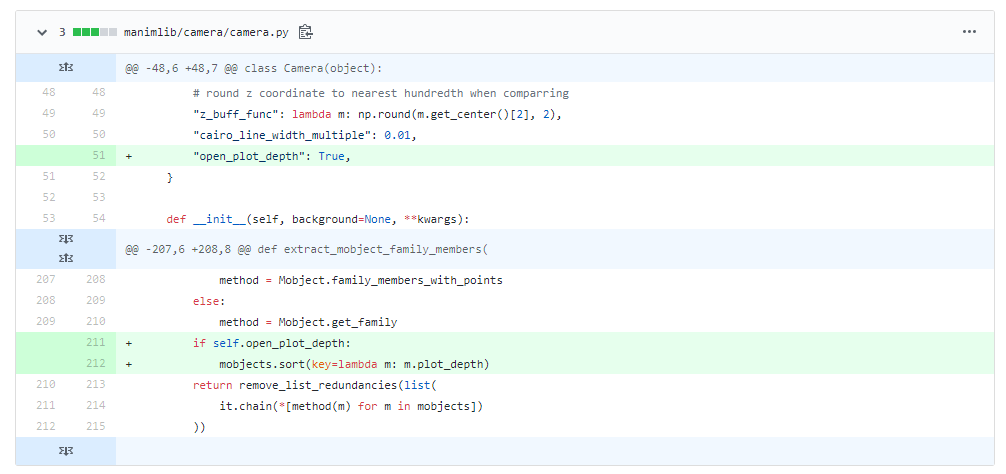
\includegraphics[width=\linewidth]{assets/pd1.png}
	\end{center}
\begin{center}
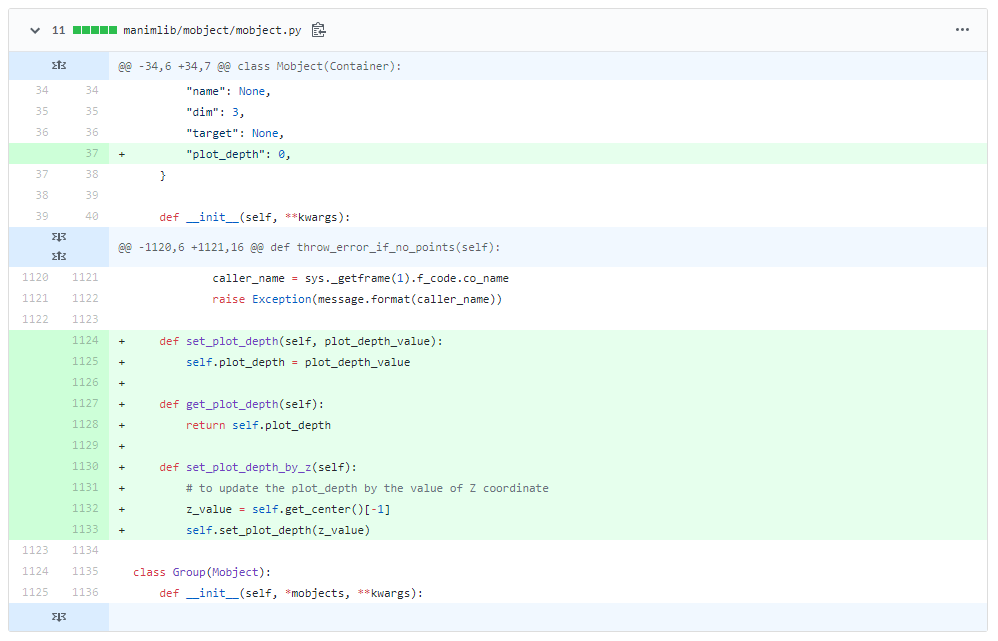
\includegraphics[width=\linewidth]{assets/pd2.png}
\end{center}
\end{figure}

\texttt{plot\_depth}的值越大,运行出来的物体就越在上面

\newpage

\subsubsection*{Q14: 如何导出\texttt{gif}文件}
\addcontentsline{toc}{subsection}{Q14: 如何导出\texttt{gif}文件}
在新版本中,\texttt{manim}导出\texttt{gif}已经失效,可以导出\texttt{mp4},后用\texttt{ffmpeg}转换。也可以按照下图修改源码
\begin{figure}[h]
	\begin{center}
		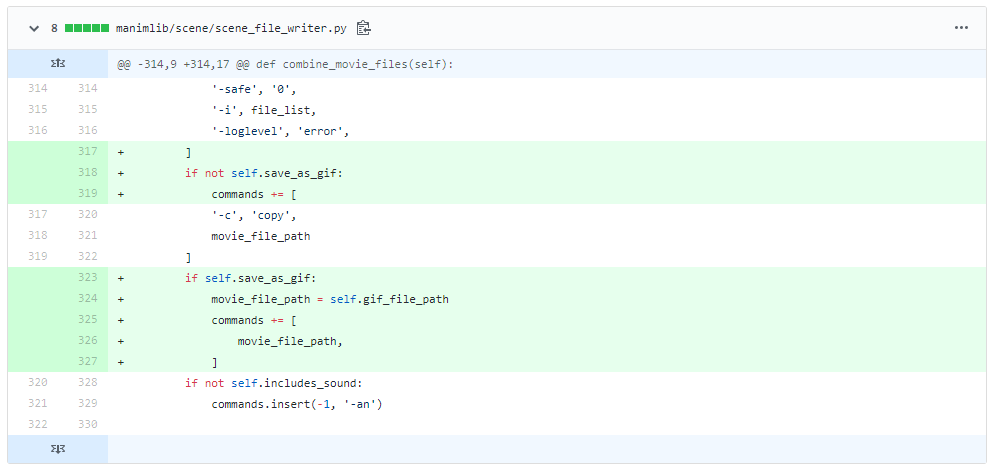
\includegraphics[width=\linewidth]{assets/gif.png}
	\end{center}
\end{figure}

改过后,在输入命令时加上\texttt{-i}选项,就能导出\texttt{gif}了

\subsubsection*{Q15: 如何导出透明的图片或者视频}
\addcontentsline{toc}{subsection}{Q15: 如何导出透明的图片或者视频}
在运行命令的时候加上 \texttt{-t}选项
\begin{itemize}
	\item 如果是 \texttt{-s}保存图片,则会存储为背景透明的\texttt{png}图片
	\item 如果是 \texttt{-l/-m/-w}保存视频,则会存储为背景透明的\texttt{mov}视频文件,方便\texttt{pr}中的剪辑
\end{itemize}

\subsubsection*{Q16: 渲染视频的画质和帧率怎么调整}
\addcontentsline{toc}{subsection}{Q16: 渲染视频的画质和帧率怎么调整}
\texttt{manim}的默认画质有四种
\begin{itemize}
	\item \texttt{-l} 最低画质 \texttt{480P15}
	\item \texttt{-m} 中等画质 \texttt{720P30}
	\item \texttt{--high\_quality}\footnote{没有缩写} 高画质 \texttt{1080P60}
	\item \texttt{-w} 导出(最高)画质 \texttt{1440P60(2K)}
\end{itemize}

不加画质选项,默认使用 \texttt{-w}最高画质\footnote{比如 \texttt{-p}(虽然很多人把 \texttt{-p}当成了 \texttt{-w}。。。)}。
可以通过修改\texttt{constants.py}中对应的画面长宽和帧率来修改\footnote{\texttt{manimlib/constants.py}的\texttt{118}行开始}

一般把 \texttt{-w}最高画质修改成\texttt{1080P60}(B站支持的最高画质)

\newpage

\subsubsection*{Q17: 有没有什么好的场景例子供学习}
\addcontentsline{toc}{subsection}{Q17: 有没有什么好的场景例子供学习}

\begin{enumerate}[1.]
	\item \texttt{Grant}的代码\footnote{\texttt{active\_projects}和\texttt{old\_projects}}对应\texttt{3B1B}的视频,可能会有报错,需要魔改
	\item 群文件里“\texttt{manim}相关的\texttt{python}代码及视频结果”
	\item 群里几个B站\texttt{up}主的\texttt{GitHub}库对应他们的代码
	\begin{itemize}
		\item \texttt{cigar666} \url{https://github.com/cigar666/my_manim_projects}
		\item 鹤翔万里 \url{https://github.com/Tony031218/manim-projects}
		\item \texttt{pdcxs} \url{https://github.com/pdcxs/ManimProjects}
		\item 有一种悲伤叫颓废 \url{https://github.com/136108Haumea/my-manim}
	\end{itemize}
\end{enumerate}


\begin{center}
    \section{注意}
\end{center}

如果有以上之外的问题,可以在群里提出,或者按照下图操作

    \begin{figure}[h]
        \begin{center}
            \includegraphics[width=6cm]{assets/grant.png}
        \end{center}
    \end{figure}

也请注意群规第 3,4 条
\begin{itemize}
    \item 3.虽为 manim 交流群,但不要一有问题就提出来,简单的问题能自己解决最好,不能解决时再寻求帮助
    \item 4.群主和管理员平时较忙,有时若不能及时回复敬请谅解
\end{itemize}

\end{document}